\chapter{Evaluation}
\label{chap:eval}
In diesem Kapitel wird die entstandene Implementierung gegen die Anforderungen verglichen und das Ergebnis evaluiert.

\section{Erfüllte Ziele}
Alle formalen Anforderungen, wie sie in Sektion \ref{sec:anforderungen} festgehalten sind, wurden erfüllt. Der Demonstrator läuft on-premise auf dem Raspberry Pi und verwaltet sämtliche Daten lokal. Es ist möglich komplexe Szenarien (Multi Event- und Action-Rules, Kontextweitergabe zwischen den Modulen, etc.) zu definieren, wobei intelligente Geräte mit Webdiensten frei zusammengefügt werden können. Dies ist möglich, da die integrierten Webservices ebenfalls als \textit{Things} im System abgebildet sind. Schließlich ist eine Benutzeroberfläche vorhanden, die es dem Nutzer erlaubt zur Laufzeit neue Szenarien zu erstellen, zu editieren und zu löschen.

\section{Vergleich mit Smart Home}
Bei dem entwickelten Demonstrator handelt es sich um eine klassische Smart Home Lösung, die auf \textit{Eclipse SmartHome} basiert und um weitere Funktionalitäten angereichert wurde. Dadurch verfügt er  über alle üblichen Funktionalitäten, die in einem Smart Home enthalten sind - er ist in der Lage ausgewählte intelligente Geräte direkt anzusteuern und in Szenarien zu automatisieren. 

\section{Vergleich mit webbasierten Task Automation Services}
%Es ist zu beachten, dass es sich bei IFTTT um einen Cloud-Service handelt. Dadurch hat es keine Möglichkeit intelligente Geräte im Haus zu steuern, sofern diese nicht über eine vom Hersteller bereitgestellte Webschnittstelle verfügen.

%In IFTTT ist es nur möglich simple Szenarien auf eine einfache Art und Weise zu definieren. Hierbei handelt es sich um sogenannte \glqq if this than that\grqq{} Szenarien, die über jeweils nur einen Trigger (\glqq this\grqq) und eine Action (\glqq that \grqq) verfügen. Der Demonstrator hingegen erlaubt es komlexe Event-Condition-Action-Regeln zu definieren.

Einen Einblick, wie sich der entstandene Demonstrator in die aktuell existierenden Task Automation Services eingliedern lässt, bietet Abbildung \ref{fig:eval0}. Wie zu sehen ist, gibt es Verbesserungen in vielen Aspekten gegenüber anderen Lösungen. Gegenüber den webbasierten TAS grenzt sich FLASH vor allem durch seine Fähigkeit ab intelligente Geräte direkt anzusteuern, sowie der deutlich mächtigeren Rule Engine ab. Es ist möglich komplexe Szenarien zu definieren, mit beliebig vielen Triggern, Bedingungen und Aktionen. Teile des Szenarios werden sequentiell abgearbeitet und können als Eingabe für spätere Elemente dienen.\\

\begin{figure}
	\centering
	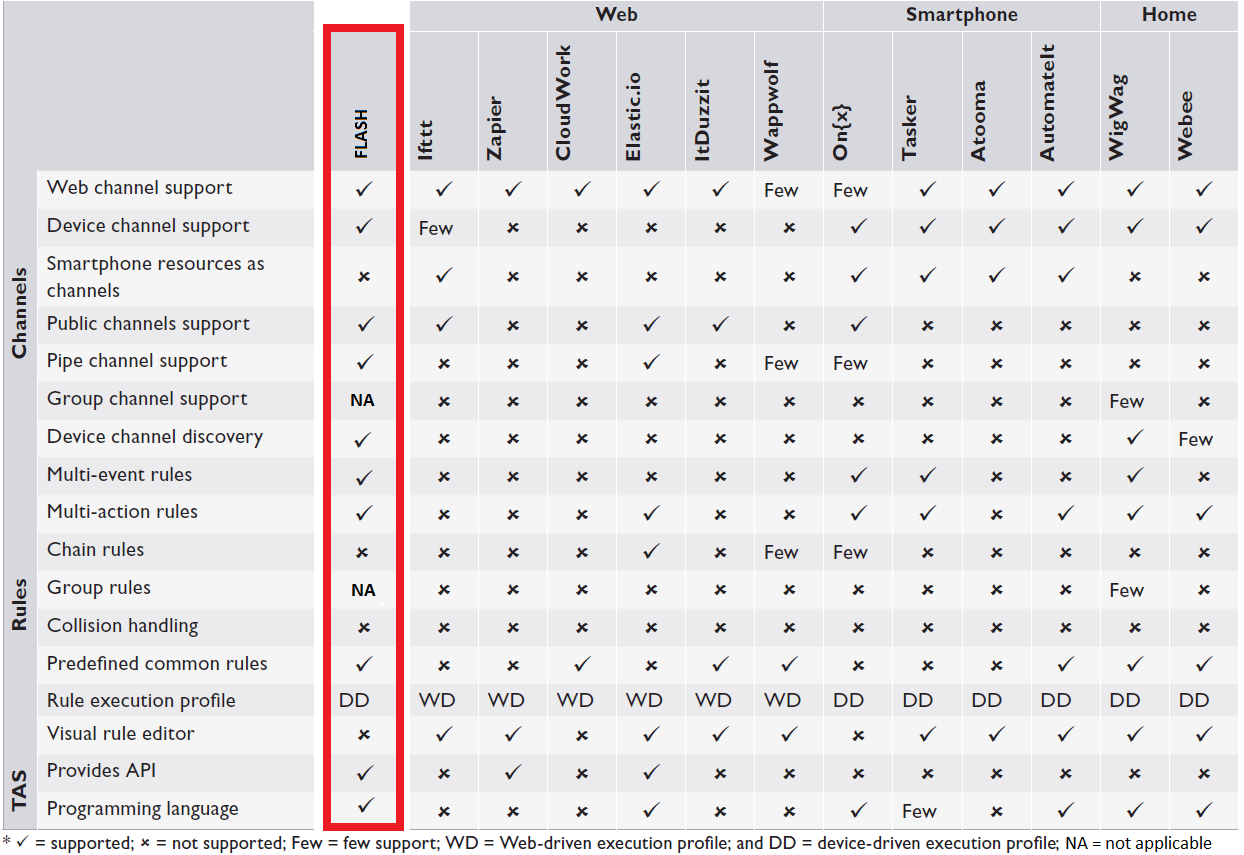
\includegraphics[width=\textwidth]{bilder/TASOverview_eval}
	\caption{Vergleich des Demonstrators mit existierenden Task Automation Services}
	\label{fig:eval0}
\end{figure}


Der entstandene Demonstrator wurde einem umfassenden Test unterzogen, im Laufe dessen Datendurchsatz und Reaktionszeiten gemessen und mit IFTTT und Zapier verglichen wurden. 

\subsection{Kopieren von Dateien in der Dropbox}
Um Durchsatz zu messen, wurde ein Szenario definiert, dass sämtliche Dateien, die in einen bestimmten Ordner in Dropbox hinzugefügt wurden, in einen anderen Ordner in der Dropbox zu kopieren. Zu Beachten ist, dass IFTTT sich auf die Abarbeitung von bis zu 15 Dateien pro Abfrage begrenzt und Dateien, die größer, als 30 MB sind, nicht beachtet. Zusätzlich wird vom Service gewarnt, dass die Ausführung aller Szenarien sich um bis zu 1 Stunde verzögern kann. Diese Tatsache führt zur Streuung, die in den nachfolgenden Grafiken festzustellen ist.

Im Falle von Zapier ist bekannt, dass nur bis zu 5 Zaps pro Abfrage alle 15 Minuten evaluiert werden. Allerdings gibt es keine Einschränkungen in der Anzahl der bearbeiteten Dateien und ihrer Größe. Aufgrund dieses Wissens wurde bei der Evaluation angenommen, dass die durchschnittliche Verzögerung der Ausführung eines Zaps bei 7,5 Minuten liegt.

Der Demonstrator lief auf einem Raspberry Pi 3 Model B, der an einen Router mit VDSL (50 MBit) Verbindung angeschlossen war.

Es wurde geprüft, wie gut die beiden Anwendungen mit einer großen Anzahl kleiner Dateien, sowie mit geringer Anzahl von großen Dateien umgehen können. 

\subsubsection{Zahlreiche kleine Dateien}
Es wurden Mengen von 258 KB großen Dateien gleichzeitig in einen Dropbox Ordner hochgeladen. Es wurden jeweils vielfache von 15 verwendet, da dies die maximale Anzahl von Dateien ist, die IFTTT in einer Abfrage bearbeitet.

Es entstanden die Grafiken \ref{fig:eval1} und \ref{fig:eval2}.
\begin{figure}
	\centering
	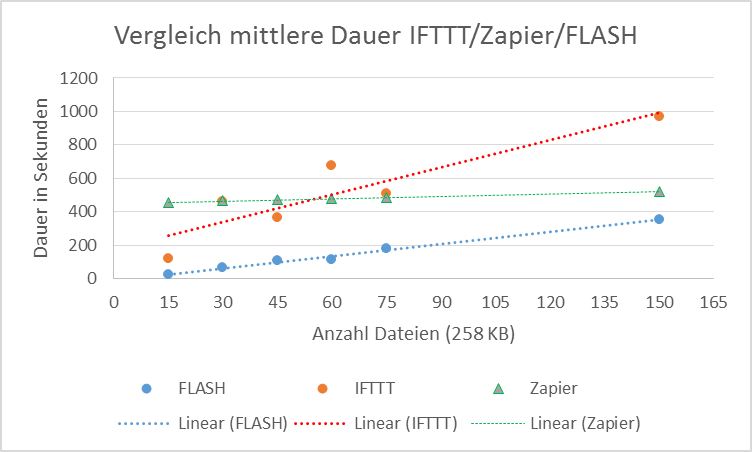
\includegraphics[width=\textwidth]{bilder/vs_mittelwert2}
	\caption{Vergleich des Mittelwerts zwischen IFTTT und FLASH für unterschiedliche Dateimengen}
	\label{fig:eval1}
\end{figure}

\begin{figure}
	\centering
	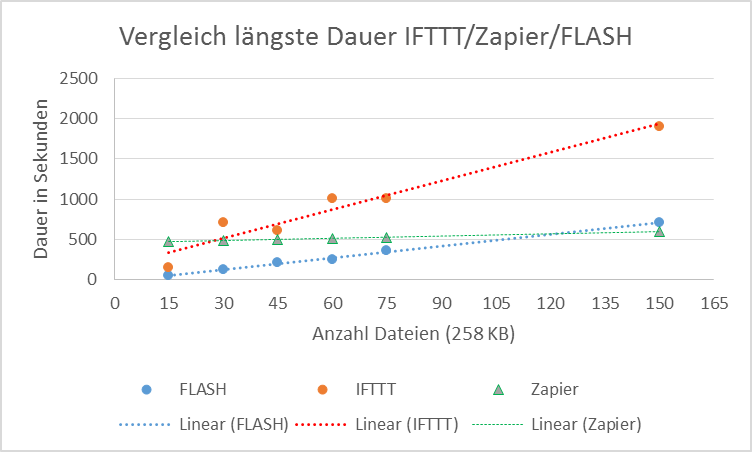
\includegraphics[width=\textwidth]{bilder/vs_laengste2}
	\caption{Vergleich der längsten Dauer (äquivalent zu Gesamtdauer, da ca. 1-2 Sekunden vernachlässigt werden können) zwischen IFTTT und FLASH für unterschiedliche Dateimengen}
	\label{fig:eval2}
\end{figure}

Für die Erstellung von Grafik \ref{fig:eval1} wurde für jede hochgeladene Datei einzeln gemessen, wie viele Sekunden es dauert, bis eine Kopie im Zielordner vorhanden ist. Es wurde anschließend ein Mittelwert gebildet und die Messung mehrmals wiederholt. Schließlich wurde ein gemeinsamer Mittelwert über die gesammelten Werte gebildet und in der Grafik für die verschiedenen Mengen von Dateien dargestellt.

In der Grafik \ref{fig:eval2} wurde analog gehandelt, mit dem Unterschied, dass hier dargestellt ist, was die längste Dauer zwischen hochladen einer Datei und der Bereitstellung der Kopie ist. Da alle Dateien nahezu gleichzeitig hochgeladen werden, kann man diesen Wert auch als Gesamtdauer, bis alle Dateien verschoben wurden, betrachten.

Bei der Messung von IFTTT wurden die berechneten Werte wie gemessen in die Grafik übertragen, da die Verzögerung vor der Ausführung des Applets unbekannt ist und nicht beeinflusst werden kann. Bei Zapier wurde hingegen eine durchschnittliche Verzögerung von 7,5 Minuten angenommen. Da es sich um kleine Dateien handelt und die Zeit, die benötigt wird um eine einzige Datei hochzuladen, vergleichbar klein ist (ca. 1 Sekunde basierend auf den gemessenen Werten) und in Betrachtung der Gesamtzeiten vernachlässigt werden kann, wurde beim Erstellen der Grafik zunächst die kleinste Zeit vom Mittelwert subtrahiert und daraufhin die erwarteten 7,5 Minuten hinzu addiert.

\subsubsection{Große Dateien}
IFTTT ist in der Lage mit Dateien umzugehen, die bis zu 30 MB groß sind. Eine Wiederholung der oben genannten Messung mit 25 MB großen Dateien hat ergeben, dass sich die Ergebnisse  analog verhalten. 

Sowohl der Demonstrator als auch Zapier sind in der Lage mit größeren Dateien umzugehen. Im Test gab es auch bei Verschiebung von 100 MB großen Dateien keinerlei Probleme.

\subsection{Steuern von Lampen bei Tweets}
Es wurde sowohl auf IFTTT als auch auf dem Demonstrator ein Szenario erstellt, dass bei jedem Tweet eine Philips Hue Lampe ausschaltet. Anschließend wurde gemessen, wie lange es dauert, bis die Lampe tatsächlich ausgeschaltet wird, nachdem der Tweet veröffentlicht wurde. Dabei steuert ITTTT die Lampe über die von Hue bereitgestellte Webschnittstelle an, während der Demonstrator das Gerät über WLAN bedient.

Es hat sich ergeben, dass die Reaktionszeit des Demonstrators stets unter einer Sekunde lag, während die Schaltung durch IFTTT eine sehr variable Dauer aufwies. Die schnellste Reaktionszeit lag bei ungefähr 10 Sekunden.

Zapier wurde in diesem Szenario nicht betrachtet, da es die Steuerung von intelligenten Geräten über vom Hersteller bereitgestellte Webdienste nicht unterstützt.


\subsection{Auswertung}
\subsubsection{Vorteile}
Aus den Messungen hat sich gezeigt, dass der Demonstrator IFTTT und Zapier in vieler Hinsicht deutlich voraus ist. Dadurch, dass er sich im Hause des Nutzers befindet, ist er in der Lage mit Geräten direkt zu kommunizieren, was der Grund für merklich bessere Reaktionszeiten in Szenarien, die intelligente Geräte im Haus betreffen, ist.\\

Auch in Szenarien, die nur Web-basiert sind und viel Download/Upload-Volumen mit sich ziehen, hat sich der Raspberry Pi als überlegen erwiesen. Dies lässt sich dadurch erklären, dass es sich bei dem Demonstrator im Gegensatz zu IFTTT und Zapier um ein dediziertes Gerät handelt, dass nur einen konkreten Nutzer bedient. Dies führt auch dazu, dass er keine arbiträren Eingrenzungen besitzt, wie z. B. die Begrenzung der Dateigröße.

Interessant ist, dass sofern Zapier keine Verzögerungen bei der Ausführung von Zaps hätte, es einen höheren Datendurchsatz aufweisen würde. Negativ an Zapier aufgefallen ist, dass es, falls es eine große Anzahl von Dateien (z. B. 150) in einem Zap bearbeiten soll, zunächst den Nutzer um eine Bestätigung bittet. Diese Bestätigung muss jedes Mal manuell erteilt werden, was die Einsatzmöglichkeiten von Zapier eingrenzt. \\

%\paragraph{Anmerkung:} Es ist zu beachten, dass diese Messung mit einem 50 MBit/s Internetanschluss erstellt wurde. Langsamere/schnellere Verbindungen könnten die Messungen entsprechend beeinflussen.\\

Schließlich ist der Raspberry Pi aus einer Datenschutzperspektive dem Cloud-Service zu bevorzugen, da sämtliche Zugriffsdaten nur lokal auf dem Gerät gesichert werden.

\subsubsection{Nachteile}
Negative Aspekte des Demonstrators sind Konsequenz der Tatsache, dass es sich dabei um eine on-premise Lösung handelt. Sämtliche Szenarien, die Webdienste automatisieren, funktionieren nur solange eine Internetverbindung  vorhanden ist. Sollte sie ausfallen, bleiben nur die charakteristischen Smart Home Funktionalitäten erhalten. In diesem Aspekt ist IFTTT dem Demonstrator voraus, da die Ausfallsicherheit in einem Rechenzentrum gegenüber der eines herkömmlichen Heimanschlusses weit überlegen ist.

Umgekehrt ist natürlich zu bedenken, dass bei einem Ausfall des Heimanschlusses auch IFTTT nicht mehr in der Lage sein wird, die hausinternen Geräte über die vom Hersteller bereitgestellten Web-Schnittstellen zu steuern. \\

Die Tatsache, dass sämtliche Zugriffsdaten auf Accounts des Users ausschließlich lokal auf dem Gerät vorhanden sind, zieht mit sich, dass im Falle eines Ausfalls (z. B. Hardware-Fehler) sämtliche Daten verloren gehen können. Dies könnte dazu führen, dass sämtliche Geräte, Dienste und Szenarien nach einer Reparatur komplett neu aufgesetzt werden müssten.



\section{Eclipse SmartHome und Quellcode}
\subsection{Positive Aspekte}
Im Laufe der Arbeit ist klar geworden, dass das Eclipse SmartHome Framework sich gut als Grundgerüst für unterschiedlichste Lösungen handelt. Die sehr generische Struktur des Frameworks hat es ermöglicht, die im Rahmen der Arbeit implementierten Funktionalitäten nahtlos in das Gesamtkonstrukt zu integrieren. 

Dies, sowie OSGi im Allgemeinen, ermöglicht es weitere Funktionalitäten (z. B. weitere Webdienste) der Anwendung hinzuzufügen, ohne bereits existierenden Code ändern zu müssen. Dank der Option, Szenarien im JSON-Format zu definieren, ist es sogar begrenzt möglich, neu hinzugefügte Webdienste in Regeln zu automatisieren, ohne die Benutzeroberfläche anzupassen.

\subsection{Negative Aspekte}
\subsubsection{Eclipse SmartHome}
Negativ aufgefallen ist die mangelnde Dokumentation von ESH, die den Einstieg in das Framework deutlich erschwert. Verstehen der einzelnen Funktionalitäten bedarf der Betrachtung des Quellcodes, wobei relevante Stellen unter den mehr als hundert Bundles erst noch identifiziert werden müssen. 

Eclipse SmartHome befindet sich derzeit noch auf Version 0.9.x und wird aktiv weiterentwickelt. Dies hat unvermeidbar dazu geführt, dass an einigen Stellen der Code nicht fehlerfrei ist. Im Laufe der Implementierung mussten an mehreren Stellen Bugs zunächst ausfindig gemacht und danach behoben werden.

\subsubsection{Quellcode}
Vor allem der Mangel eines visuellen Regeleditors begrenzt derzeit die Nutzungsmöglichkeiten des Demonstrators. Zwar ist es möglich, Szenarien zur Laufzeit zu editieren, so bedarf dies dennoch Kenntnissen von JSON, sowie den existierenden Event-Typen, sowie der Eingaben und Ausgaben von Triggern, Bedingungen und Aktionen.

\section{Fazit}
Die Implementierung erfüllt alle explizit definierten Anforderungen an die Funktionsweise und weist deutliche Verbesserungen in wesentlichen Aspekten gegenüber der Konkurrenz auf. Sie lässt sich leicht um neue Elemente und Funktionalitäten erweitern.

